\documentclass[a4paper,12pt]{article}
\usepackage{cmap}
\usepackage[T2A]{fontenc}
\usepackage[utf8]{inputenc}
\usepackage[english,russian]{babel}
\usepackage{listings}
\usepackage{amsmath}
\usepackage{float}
\usepackage{csquotes}
\usepackage{graphicx}
\usepackage{xcolor}
\usepackage{hyperref}
\usepackage{mathtools}

\renewcommand{\theequation}{\thesection.\arabic{equation}}


\author{Шерепа Никита}
\title{ThinkDSP. Лабораторная 4. Шум.}
\date{\today}

\graphicspath{{res/screenshots}}

\begin{document}%
	
	\maketitle
	
	\newpage \tableofcontents
	\newpage \listoffigures
	\newpage \lstlistoflistings
	
	\newpage
	
	\definecolor{dkgreen}{rgb}{0,0.6,0}
	\definecolor{gray}{rgb}{0.5,0.5,0.5}
	\definecolor{mauve}{rgb}{0.58,0,0.82}
	
	\lstset{
		language=Python,                 % выбор ЯП для подсветки 
		basicstyle=\small\sffamily, % размер и начертание шрифта для подсветки кода
		numbers=left,               % где поставить нумерацию строк (слева\справа)
		numberstyle=\tiny,           % размер шрифта для номеров строк
		stepnumber=1,                   % размер шага между двумя номерами строк
		numbersep=5pt,                % как далеко отстоят номера строк от подсвечиваемого кода
		aboveskip=3mm,
		belowskip=3mm,
		showstringspaces=false,
		columns=flexible,
		captionpos=b, 
		basicstyle={\small\ttfamily},
		numbers=left,
		numberstyle=\tiny\color{gray},
		keywordstyle=\color{blue},
		commentstyle=\color{mauve},
		stringstyle=\color{dkgreen},
		breaklines=true,
		breakatwhitespace=true,
		tabsize=3
	}

	\section{Упражнение 4.1}
	
	\begin{enumerate}
		
		\item \textbf{Задание}
		
		Скачайте несколько файлов с веб-страницы \textit{http://asoftmurmur.com/about/]} и вычислисте спектры каждого сигнала. Похож ли спетр мощности на белый, розовый или броуновский шум? Как спектр меняется во времени?
		
		\item \textbf{Ход работы}
		
		Я скачал несколько звуков. Начнем со звука морских волн. Воспроизведем его, выделим сегмент и построим его спектр. 
		\begin{lstlisting}[caption=Работа со звуком морских волн]
			import numpy as np
			import matplotlib.pyplot as plt
		
			from thinkdsp import decorate
			from thinkdsp import read_wave
			
			wave = read_wave('res/audio/Sea_waves.wav')
			wave.make_audio()
			segment = wave.segment(start=20, duration=3.0)
			segment.make_audio()
			
			spectrum = segment.make_spectrum()
			spectrum.plot_power()
			decorate(xlabel='Frequency (Hz)')
		\end{lstlisting}
		\begin{figure}[H]
			\centering
			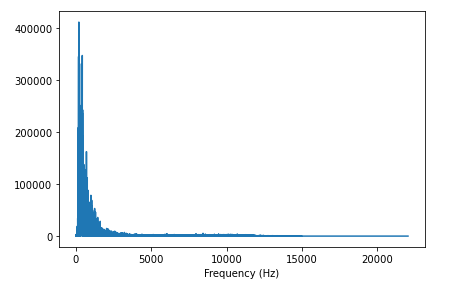
\includegraphics[width=0.75\textwidth]{1_1.png}
			\caption{Спектр сегмента}
			\label{fig:1.1}
		\end{figure}
		
		Видим, что амлитуда убывает с частотой. Поэтому это может быть или броуновский (красный) или розовый шум. Построим спектр мощности на логарифмической шкале.
		
		\begin{lstlisting}[caption=Спектр мощности]
			spectrum.plot_power()
			
			loglog = dict(xscale='log', yscale='log')
			decorate(xlabel='Frequency (Hz)', **loglog)
		\end{lstlisting}
		\begin{figure}[H]
			\centering
			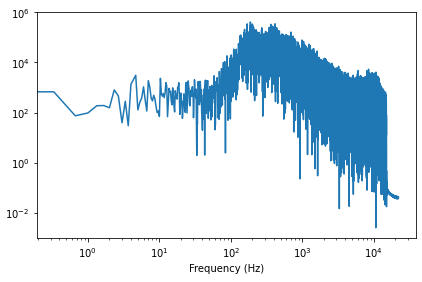
\includegraphics[width=0.75\textwidth]{1_2.png}
			\caption{Спектр мощности}
			\label{fig:1.2}
		\end{figure}
		
		Из-за увеличения и уменьшения амплитуды это все выглядит как стандартный и естественный источник шума.
		
		Выберем другой звук - сверчки. Воспроизведем его, выделим сегмент и построим его спектр. 
		
		\begin{lstlisting}[caption=Работа со звуком сверчков]
			wave = read_wave('res/audio/crickets_texas.wav')
			wave.make_audio()
		\end{lstlisting}
		\begin{figure}[H]
			\centering
			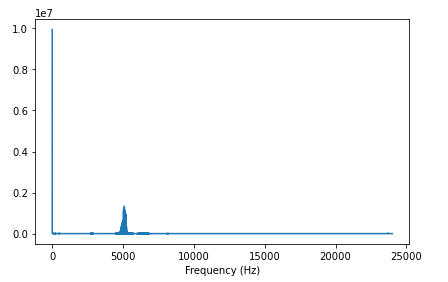
\includegraphics[width=0.75\textwidth]{1_3.png}
			\caption{Спектр сегмента}
			\label{fig:1.3}
		\end{figure}
		
		Немного приблизим
		\begin{lstlisting}[caption=Приближаем спектр]
			spectrum = wave.segment(start = 0, duration = 5).make_spectrum()
			spectrum.high_pass(100)
			spectrum.plot()
		\end{lstlisting}
		\begin{figure}[H]
			\centering
			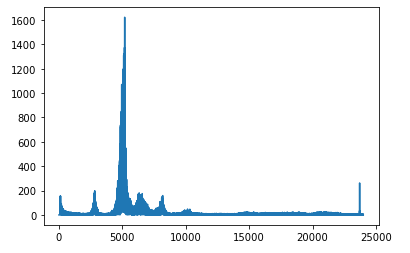
\includegraphics[width=0.75\textwidth]{1_4.png}
			\caption{Приближенный спектр сегмента}
			\label{fig:1.4}
		\end{figure}
		
		Видим, что по характеру изменения частот это не похрже ни на белый шум, ни на розовый
		
		Построим спектр мощности на логарифмической шкале.
		\begin{lstlisting}[caption=Спектр мощности]
			spectrum.plot_power()
			
			loglog = dict(xscale='log', yscale='log')
			decorate(xlabel='Frequency (Hz)', **loglog)
		\end{lstlisting}
		\begin{figure}[H]
			\centering
			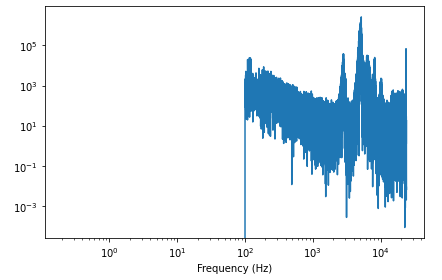
\includegraphics[width=0.75\textwidth]{1_5.png}
			\caption{Спектр мощности}
			\label{fig:1.5}
		\end{figure}
		
		Теперь построим спектрограмму
		\begin{lstlisting}[caption=Построение спектрограммы звука сверчков]
			segment.make_spectrogram(512).plot(high=5000)
			decorate(xlabel='Time(s)', ylabel='Frequency (Hz)')
		\end{lstlisting}
		\begin{figure}[H]
			\centering
			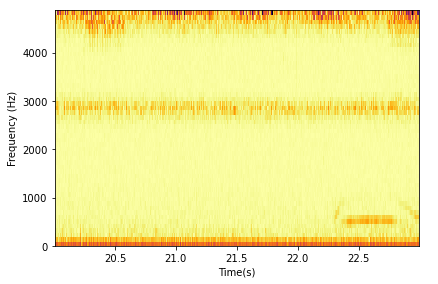
\includegraphics[width=0.75\textwidth]{1_6.png}
			\caption{Спектрограмма звука сверчков}
			\label{fig:1.5}
		\end{figure}
		
		Исходя из спектра мощности и спектрограммы, звук сверчков можно назвать шумом, похожим на белый.
		
	\end{enumerate}
	\newpage
	
	
	\section{Упражнение 4.2}
	
	\begin{enumerate}
		
		\item \textbf{Задание}
		
		Реализуйте метод Бартлетта и используйте его для оценки спектра мощности шумового сигнала.
		
		\item \textbf{Ход работы}
		
		Реализуем метод Бартлетта
		\begin{lstlisting}[caption=Метод Бартлетта]
			from thinkdsp import Spectrum
			
			def bartlett_method(wave, seg_length=512, win_flag=True):
			spectro = wave.make_spectrogram(seg_length, win_flag)
			spectrums = spectro.spec_map.values()
			
			psds = [spectrum.power for spectrum in spectrums]
			
			hs = np.sqrt(sum(psds) / len(psds))
			fs = next(iter(spectrums)).fs
			
			spectrum = Spectrum(hs, fs, wave.framerate)
			return spectrum
		\end{lstlisting}
	
		Теперь возьмем сегмент звука морской волны и применим к нему метод Бартлетта
		
		\begin{lstlisting}[caption=Применение метода Бартлетта]
			wave = read_wave('res/audio/Sea_waves.wav')
			
			segment = wave.segment(start=10, duration=3.0)
			segment.make_audio()
			
			psd = bartlett_method(segment)
			
			psd.plot_power()
			
			decorate(xlabel='Frequency (Hz)', 
			ylabel='Power', 
			**loglog)
		\end{lstlisting}
		\begin{figure}[H]
			\centering
			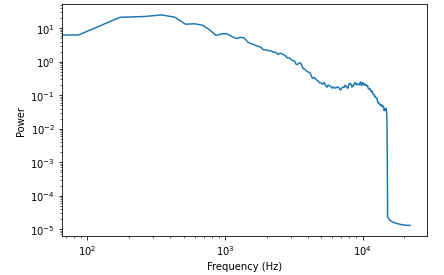
\includegraphics[width=0.75\textwidth]{2_1.png}
			\caption{Спектр сегмента}
			\label{fig:2.1}
		\end{figure}
			
		Видим, что сигнал стабильный. Зависимости более менее одинаковая для разных моментов времени.
		
	\end{enumerate}
	\newpage
	
	
	\section{Упражнение 4.3}
	
	\begin{enumerate}
		
		\item \textbf{Задание}
		
		Откройте файл с историческими данными о ежедневной цене BitCoin и вычислите спектр цен BitCoin как функцию времени. Похоже ли это на белый, розовый или броуновский шум?
		
		
		\item \textbf{Ход работы}
		
		Посмотрим динамику цен BitCoin за последние 7 лет.
		
		\begin{lstlisting}[caption=Считывание динамики цен BitCoin]
			import pandas as pd
			
			df = pd.read_csv('res/BTC_USD_2013-10-01_2021-05-05-CoinDesk.csv', 
			parse_dates=[0])
			df
		\end{lstlisting}
		\begin{figure}[H]
			\centering
			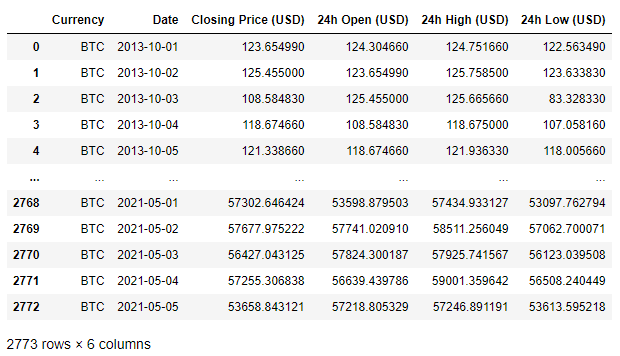
\includegraphics[width=0.75\textwidth]{3_1.png}
			\caption{Динамика цен BitCoin}
			\label{fig:3.1}
		\end{figure}
		
		Теперь построим график, для большей наглядности
		\begin{lstlisting}[caption=Построение графика цен BitCoin]
			ys = df['Closing Price (USD)']
			ts = df.index
			
			from thinkdsp import Wave
			
			wave = Wave(ys, ts, framerate=1)
			wave.plot()
			decorate(xlabel='Time (days)')
		\end{lstlisting}
		\begin{figure}[H]
			\centering
			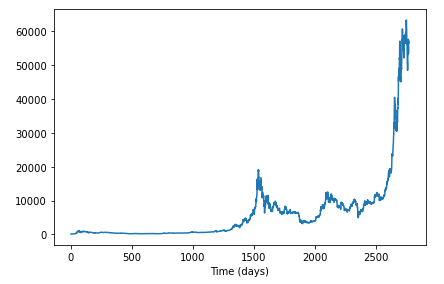
\includegraphics[width=0.75\textwidth]{3_2.png}
			\caption{График цен BitCoin}
			\label{fig:3.2}
		\end{figure}
		
		Построим спектр мощности на логарифмической шкале.
		\begin{lstlisting}[caption=Спектр мощности]
			spectrum = wave.make_spectrum()
			spectrum.plot_power()
			decorate(xlabel='Frequency (1/days)', **loglog)
		\end{lstlisting}
		\begin{figure}[H]
			\centering
			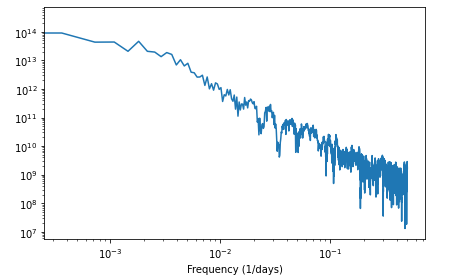
\includegraphics[width=0.75\textwidth]{3_3.png}
			\caption{Спектр мощности}
			\label{fig:3.3}
		\end{figure}
		
		Вычислим наклон прямой
		\begin{lstlisting}[caption=Спектр мощности]
			spectrum.estimate_slope()[0]
			
			Output
			-1.8717417425660792
		\end{lstlisting}
		
		Наклон = -1.8717417425660792.
		
		Как видим, результат похож на розовый шум (наклон лежит в диапазоне от |0| до |2|)
		
	\end{enumerate}
	\newpage


	\section{Упражнение 4.4}
	
	\begin{enumerate}
		
		\item \textbf{Задание}
		
		Напишите класс, называемый \textit{UncorrelatedPoissonNoise}, наследующий \textit{thinkdsp.\_Noise} и предоставляющий \textit{evaluate}. Следует использовать \textit{Np.random.poisson} для генерации случайных величин из распределения Пуассона. Параметр этой функции \textit{lam} - это среднее число частиц за время каждого интервала. Можно использовать атрибут \textit{amp} для определения \textit{lam}. Например, при частоте кадров 10 кГц и \textit{amp} 0.001 получится около 10 "щелчков" (как у счетчика Гейгера) в секунду.
		
		Сгенерируейте пару секунд UP и прослушайте. Для малых значений \textit{amp}, например 0.001, звук будет как у счетчика Гейгера. При больших значениях он будет похож на белый шум. Вычислите и напечатайте спектр мощности и посмотрите, так ли это.
		
		
		\item \textbf{Ход работы}
		
		Реализуем класс \textit{UncorrelatedPoissonNoise}
		\begin{lstlisting}[caption=Класс UncorrelatedPoissonNoise]
			from thinkdsp import Noise
			
			class UncorrelatedPoissonNoise(Noise):
			
				def evaluate(self, ts):
				ys = np.random.poisson(self.amp, len(ts))
			return ys
		\end{lstlisting}
		
		Теперь создадим и прослушаем UP
		\begin{lstlisting}[caption=Создание и воспроизведение UP]
			amp = 0.001
			framerate = 10000
			duration = 1
			
			signal = UncorrelatedPoissonNoise(amp=amp)
			wave = signal.make_wave(duration=duration, framerate=framerate)
			wave.make_audio()
		\end{lstlisting}
		
		Звучик как "щелчки" счетчика Гейгера.
		
		Сравним ожидаемое количество частиц с получившимся
		\begin{lstlisting}[caption=Создание и воспроизведение UP]
			expected = amp * framerate * duration
			actual = sum(wave.ys)
			print(expected, actual)
			
			
			Output
			10.0 10
		\end{lstlisting}
		
		Видим, что все совпало.
		
		Теперь визуализируем полученный звук
		\begin{lstlisting}[caption=Визуализация щелчков]
			wave.plot()
		\end{lstlisting}
		\begin{figure}[H]
			\centering
			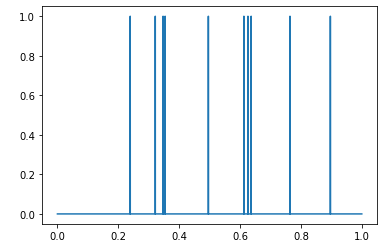
\includegraphics[width=0.75\textwidth]{4_1.png}
			\caption{Визуализация щелчков}
			\label{fig:4.1}
		\end{figure}
		
		Построим спектр мощности на логарифмической шкале.
		\begin{lstlisting}[caption=Спектр мощности]
			spectrum = wave.make_spectrum()
			spectrum.plot_power()
			decorate(xlabel='Frequency (1/days)', **loglog)
		\end{lstlisting}
		\begin{figure}[H]
			\centering
			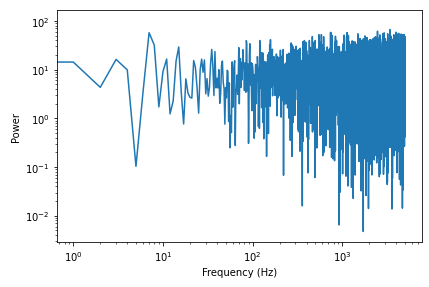
\includegraphics[width=0.75\textwidth]{4_2.png}
			\caption{Спектр мощности}
			\label{fig:4.2}
		\end{figure}
		
		Вычислим наклон.
		\begin{lstlisting}[caption=Вычисление наклона]
			spectrum.estimate_slope().slope
			
			Output
			-0.0003900929448715259
		\end{lstlisting}
		
		Похоже на белый шум.
		
		
		Теперь увеличим амлитуду сигнала - amp, и посмотрим что будет.
		\begin{lstlisting}[caption=Создание\, вопроизведение и построение графика нового звука]
			amp = 1
			framerate = 10000
			duration = 1
			
			signal = UncorrelatedPoissonNoise(amp=amp)
			wave = signal.make_wave(duration=duration, framerate=framerate)
			wave.make_audio()
			wave.plot()
		\end{lstlisting}
		\begin{figure}[H]
			\centering
			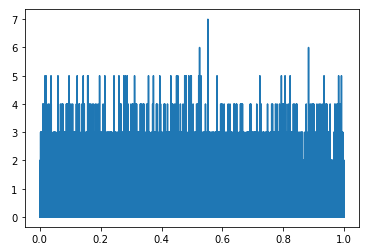
\includegraphics[width=0.75\textwidth]{4_3.png}
			\caption{График нового звука}
			\label{fig:4.3}
		\end{figure}
	
		Спектр сходится на Гауссовском шуме.
		
		Теперь сравним спектры
		\begin{lstlisting}[caption=Сравнение спектров]
			amp = 1
			framerate = 10000
			duration = 1
			
			signal = UncorrelatedPoissonNoise(amp=amp)
			wave = signal.make_wave(duration=duration, framerate=framerate)
			wave.make_audio()
			wave.plot()
		\end{lstlisting}
		\begin{figure}[H]
			\centering
			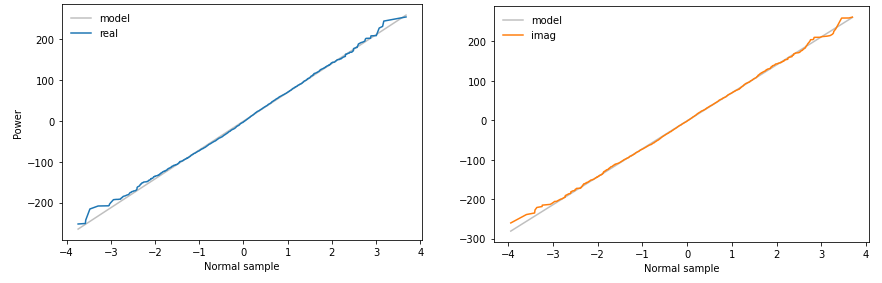
\includegraphics[width=0.75\textwidth]{4_4.png}
			\caption{Сравнение спектров}
			\label{fig:4.4}
		\end{figure}
		
	\end{enumerate}
	\newpage
	
	
	\section{Упражнение 4.5}
	
	\begin{enumerate}
		
		\item \textbf{Задание}
		
		Изучите алгоритм Восса-МакКартни для генерации розового шума, реализуйте его, вычислите спектр результата и убедитесь, что соотношение между мощностью и частотой соответсвующее.
		
		\item \textbf{Ход работы}
		
		Напишем функцию для реализации алгоритма Восса-МакКартни
		\begin{lstlisting}[caption=Алгоритм ВОсса-МакКартни]
			def voss(nrows, ncols=16):
				array = np.empty((nrows, ncols))
				array.fill(np.nan)
				array[0, :] = np.random.random(ncols)
				array[:, 0] = np.random.random(nrows)
				
				# the total number of changes is nrows
				n = nrows
				cols = np.random.geometric(0.5, n)
				cols[cols >= ncols] = 0
				rows = np.random.randint(nrows, size=n)
				array[rows, cols] = np.random.random(n)
				
				df = pd.DataFrame(array)
				df.fillna(method='ffill', axis=0, inplace=True)
				total = df.sum(axis=1)
				
				return total.values
		\end{lstlisting}
		
		Для проверки сгенерируем 12005 значений
		\begin{lstlisting}[caption=Генерация значений]
			ys = voss(11025)
			ys
			
			Output
			array([7.79201163, 7.35145659, 7.20205832, ..., 9.22659538, 8.72048853,
			9.15790613])
		\end{lstlisting}
	
		Теперь создадим из этих значений звук и визуализиуем его.
		\begin{lstlisting}[caption=Создание и визуализация звука]
			ys = voss(11025)
			ys
			
			Output
			array([7.79201163, 7.35145659, 7.20205832, ..., 9.22659538, 8.72048853,
			9.15790613])
		\end{lstlisting}
		\begin{figure}[H]
			\centering
			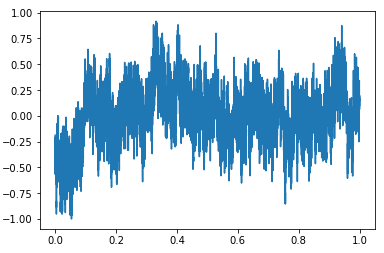
\includegraphics[width=0.75\textwidth]{5_1.png}
			\caption{Визуализация звука}
			\label{fig:5.1}
		\end{figure}
		
		Разброс частот слишком большой для белого шума.
		
		Построим спектр мощности на логарифмической шкале.
		\begin{lstlisting}[caption=Спектр мощности]
			spectrum = wave.make_spectrum()
			spectrum.hs[0] = 0
			spectrum.plot_power()
			decorate(xlabel='Frequency (Hz)',
			**loglog)
		\end{lstlisting}
		\begin{figure}[H]
			\centering
			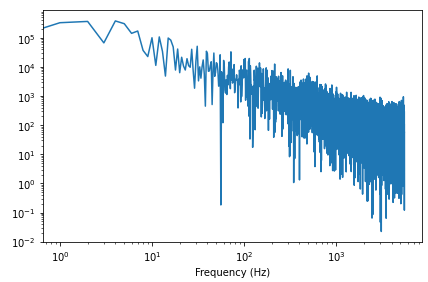
\includegraphics[width=0.75\textwidth]{5_2.png}
			\caption{Спектр мощности}
			\label{fig:5.2}
		\end{figure}
		
		Вычислим наклон
		\begin{lstlisting}[caption=Вычисление наклона]
			spectrum.estimate_slope().slope
			
			Output
			-0.9885351381362323
		\end{lstlisting}
	
		Наклон = -0.9885351381362323
		
		Попробуем получить более точные данные среднего спектра мощности.
		
		Сгенерируем большую выборку, затем с помощью метода Бартлетта вычислим значения и построим график спектра мощности
		\begin{lstlisting}[caption=Уточнение результата]
			seg_length = 64 * 1024
			iters = 100
			wave = Wave(voss(seg_length * iters))
			len(wave)
			
			spectrum = bartlett_method(wave, seg_length=seg_length, win_flag=False)
			spectrum.hs[0] = 0
			len(spectrum)
			
			spectrum.plot_power()
			decorate(xlabel='Frequency (Hz)',
			**loglog)
		\end{lstlisting}
		\begin{figure}[H]
			\centering
			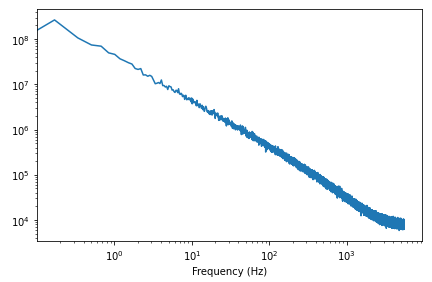
\includegraphics[width=0.75\textwidth]{5_3.png}
			\caption{Более точный спектр мощности}
			\label{fig:5.3}
		\end{figure}
		
		Пересчитаем наклон
		\begin{lstlisting}[caption=Пересчитывание наклона]
			spectrum.estimate_slope().slope
			
			Output
			-1.0018254851474162
		\end{lstlisting}
		
		Наклон = -1.0018254851474162
		
		Основываясь на всех полученных результатах выше, можно сказать, что перед нам розовый шум.
		
	\end{enumerate}
	\newpage
	
	
	\section{Вывод}
	
	В результате выполнения лабораторной работы получены навыки работы с шумами. Были изучены разные виды шумов: белый, красный, розовый. Также были изучены такие алгоритмы обработки шумов как метот Бартлетта и алгоритм Восса-МакКартни.


\end{document}